\chapter{State of the Art}
\label{cha:state_of_art}

\begin{itemize}
    \item Zoom out history \cite{Deamer2016}
\end{itemize}




\section{Nanopore Sequencing in the Literature}
\label{sec:state_of_art:nanopore_literature}

\begin{itemize}
    \item Motivation: Too many publications to read, too fast progress to stay up to date
    \item Motivation: OpenSyllabusGallxy visualizing books read in NA universities.
    \item Introduce S2ORC dataset, summary, paper, journals, topics
    \item Complement with Crossref API
    \item Plot UMAP of all publications, highlight 'nanopore cluster'
    %\item paper over time, impact (over time?) topics
    \item wordclouds or timeline to illustrate usage of the technology
    \item most impact by incoming citations, normalized by year/age
    \item missing but relevant publications for this work, limitations of computational literature scan
\end{itemize}




\section{\Biorxiv\ Preprints}
\label{sec:state_of_art:biorxiv}

\begin{itemize}
    \item Role of preprints for nanopore, bioRxiv as platform
    \item stats of bioRxiv, paper, topics, nanopore paper, publication rate and impact
    \item Example of read-until, visible for in-field experts, hidden for outsider?
    \item Comment/Opinion on preprints in fast-moving fields, coronavirus example, weight potential against risks
    \item Mention Twitter as fast but also least reliable source
\end{itemize}




\section{Throughput and Accuracy}
\label{sec:stat_of_art:throughput}

\begin{itemize}
    \item Representative Flow-Cells over time (from 3 to 30 GBp in 48h)
    \item Size selection, shearing, nuclease flush
    \item accuracy guppy-fast, guppy-hac (mention albacore flappie, scrappie, SACall, chiron, ...)
    \item cite benchmark paper, illustrate need for in-house benchmark of each new version
    \item Mapping of long reads depending on genomic context, read length, Q-Score etc.
    \item Accuracy of base modifications: Nanopolish, Signalign, DeepMod, DeepSignal etc.
    %\item Nanopolish context and signal level analysis
\end{itemize}

\begin{figure}[h]
    \centering
    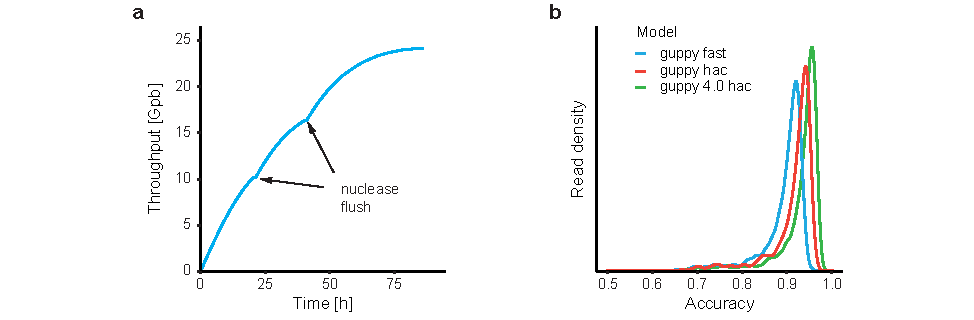
\includegraphics[width=1.0\textwidth]{figures/state_of_art/throughput.pdf}
    \captionsetup{format=plain}
    \caption[Throughput and accuracy]{Throughput and single read accuracy. \textbf{a}, Cumulative sequencing throughput over time of one representative MinION flow cell. Nuclease flushes unblock clogged pores and reload the flow cell with a new library. \textbf{b}, Density plot comparing single read accuracy (BLAST identiy) of 4k random reads basecalled with fast and high-accuracy model of \textit{Guppy} v3.5 and high-accuracy model of \textit{Guppy} v4.0 (Median accuracy: 0.90, 0.93, 0.95; Modal: 0.92, 0.94, 0.95).}
    \label{fig:state_of_art:throughput}
\end{figure}

\begin{figure}[h]
    \centering
    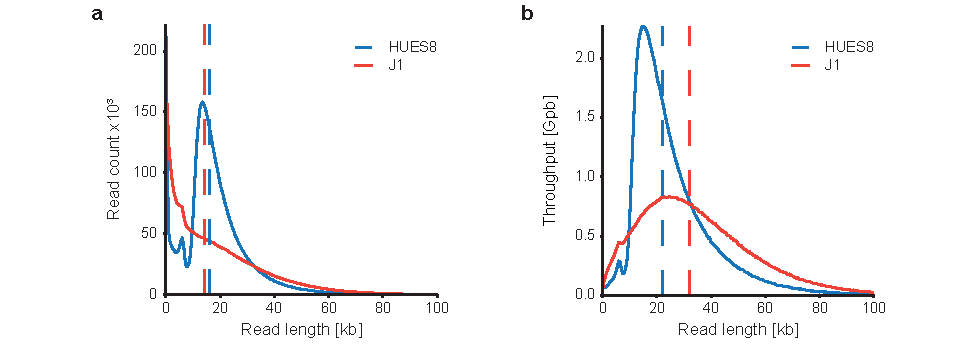
\includegraphics[width=1.0\textwidth]{figures/state_of_art/read_length.pdf}
    \captionsetup{format=plain}
    \caption[Read length median and N50]{Read length distribution: \textbf{a}, Read length distributions shown as number of reads per length (bins of 500nt) of two PromethION flow cells loaded with libraries from different DNA extraction methods. Dashed lines show median read length at 15883 (HUES8) and 14281 (J1). \textbf{b}, Read length distributions shown as sequenced basepairs per read length. Dashed lines show N50 at 21041 (HUES8) and 31906 (J1).}
    \label{fig:state_of_art:read_length}
\end{figure}